\section{Rigidity of the family: local dimension and compatibility radius}\label{sec:rigidity}

We now show that the adaptive Pauli strategy of Section~\ref{sec:iteration} is optimal on $G_{j,R}$ and $S^j_\lambda(K_3)$ in two strong senses. First, every finite-dimensional quantum $3$-coloring of either graph has local dimension divisible by $4^j$; this uses only the edge rule and no compatibility condition. Second, no quantum $3$-coloring of either graph is $k$-compatible for any $k>\max\{R,2\}$. At the end of Section~\ref{sec:largest-radius}, these results combine with Section~\ref{sec:iteration} to complete the proof of Theorem~\ref{thm:main}.

\subsection{Coordinate projections and edge transport}\label{sec:coord-proj}

\begin{theorem}\label{thm:dimension}
Let $j,R\ge1$ and $\lambda=\max\{R-2,0\}$. Every finite-dimensional quantum $3$-coloring of $G_{j,R}$, and hence of $S^j_\lambda(K_3)$, has local dimension divisible by $4^j$. For either graph, the local dimensions of the $R$-compatible quantum $3$-colorings are exactly the positive multiples of $4^j$.
\end{theorem}

Throughout this section, $(P_{v,a})_{a\in\mathbb Z/3}$ is an arbitrary finite-dimensional quantum $3$-coloring of $G_{j,R}$ on $\C^d$. The displayed strategy~\eqref{eq:strategy} selects one of four input positions in each basis. We show that the projectors of every quantum $3$-coloring split $\C^d$ in the same way, into four subspaces of equal dimension at each of the $j$ levels.

Recall that the categorical power $K_3^{\times m}$ has vertex set $(\mathbb Z/3)^m$, with two words adjacent precisely when they differ in every coordinate. Pulling back $(P_{v,a})$ along any graph homomorphism $F:K_3^{\times m}\to G_{j,R}$ yields a quantum $3$-coloring $(P_{F(u),a})$ of $K_3^{\times m}$. Every such coloring decomposes into summands that depend on a single coordinate.

\begin{lemma}[Coordinate decomposition]\label{lem:k3-powers}
In a quantum $3$-coloring $(P_{u,a})$ of $K_3^{\times m}$ on $\C^d$ all projectors commute. There is an orthogonal decomposition $\C^d=V_1\oplus\cdots\oplus V_m$ that reduces every projector, such that on $V_i$ the measurement at $u$ depends only on $u_i$ and, as a function of $u_i$, satisfies the edge rule of $K_3$.
\end{lemma}

The self-contained analytical proof of Lemma~\ref{lem:k3-powers} is given in Appendix~\ref{app:k3-powers}. (The statement is the case $n=3$ of~\cite[Theorem~7.1]{CvdDZ}, which is not imported here.)

Given a graph homomorphism $F:K_3^{\times m}\to G_{j,R}$ and a subset $B\subseteq\{1,\ldots,m\}$ of input coordinates, two measurements determine the orthogonal projection onto $\bigoplus_{i\in B} V_i$. Writing $\mathbf 1\in(\mathbb Z/3)^m$ for the all-one word and $\mathbf 1_B\in(\mathbb Z/3)^m$ for the word equal to $1$ on $B$ and $0$ outside $B$, define the \emph{coordinate projection} of $B$ by
\begin{equation}\label{eq:coordinate-projection}
 S_F(B)=\sum_{a\in\mathbb Z/3} P_{F(\mathbf 1),a}\,P_{F(\mathbf 1_B),a}.
\end{equation}
The proofs of this section rest on seven facts, which we collect here. The first two concern presentation trees, the next three coordinate projections, and the last two compare the measurements at different vertices.
\begin{list}{}{\setlength{\labelwidth}{3.6em}\setlength{\labelsep}{0.6em}\setlength{\leftmargin}{4.2em}\setlength{\itemsep}{3pt}\setlength{\parsep}{0pt}\setlength{\topsep}{4pt}}
\item[\textup{Fact 1.}] \emph{Trees give homomorphisms.} A presentation tree with its root at level $j$ that meets the bounds of Definition~\ref{def:sparse-graph}, with independent variables in $\mathbb Z/3$ assigned to its leaves, defines a graph homomorphism from a categorical power of $K_3$ into $G_{j,R}$. Indeed, changing every leaf variable yields adjacent vertices at level $0$, and each basis node or wire node preserves coordinatewise adjacency at every level. The same holds if several leaves carry the same variable.
\item[\textup{Fact 2.}] \emph{Consecutive layers.} Two graph homomorphisms $F,F':K_3^{\times m}\to G_{j,R}$ satisfy the \emph{cross-edge condition} if $F(u)\sim F'(v)$ whenever $u,v\in(\mathbb Z/3)^m$ differ in every coordinate. This holds for the homomorphisms of two trees as in Fact~1 that are identical except for the layer indices at a single wire node, if these two indices are consecutive. The reason is the same as in Fact~1, because two vertices in consecutive layers of a wire are adjacent whenever both of their entries are adjacent.
\item[\textup{Fact 3.}] \emph{Coordinate projections.} The operator $S_F(B)$ is the orthogonal projection onto $\bigoplus_{i\in B}V_i$. Indeed, on a summand $V_i$ with $i\in B$, the words $\mathbf 1$ and $\mathbf 1_B$ agree in coordinate $i$, so $P_{F(\mathbf 1),a}$ and $P_{F(\mathbf 1_B),a}$ coincide on $V_i$, and the sum of their products over $a$ is the identity on $V_i$. On $V_i$ with $i\notin B$, the two words differ in coordinate $i$, so every term $P_{F(\mathbf 1),a}P_{F(\mathbf 1_B),a}$ vanishes on $V_i$ by the edge rule of $K_3$. In particular, disjoint sets of coordinates yield orthogonal projections, and $S_F(\{1,\ldots,m\})=I$.
\item[\textup{Fact 4.}] \emph{Other pairs of words.} By the same argument, $\mathbf 1$ and $\mathbf 1_B$ may be replaced in~\eqref{eq:coordinate-projection} by any two words that agree on $B$ and differ in every coordinate outside $B$.
\item[\textup{Fact 5.}] \emph{Identifying variables.} If some of the input variables are set equal to one another, the coordinate projection of the resulting variable is the sum of their coordinate projections, and the coordinate projections of the other variables do not change. This follows from the definition~\eqref{eq:coordinate-projection} and Fact~3, because identifying variables turns the words $\mathbf 1$ and $\mathbf 1_B$ into words of the same form.
\item[\textup{Fact 6.}] \emph{Triangle identity.} On any triangle $\{u,v,w\}$ of a graph with a quantum $3$-coloring, the three projectors for a fixed color $a$ are pairwise orthogonal, so $P_{u,a}+P_{v,a}+P_{w,a}\le I$. Summing this inequality over the three colors gives $3I\le3I$, which forces equality:
\[
 P_{u,a}+P_{v,a}+P_{w,a}=I\qquad\text{for every color }a.
\]
\item[\textup{Fact 7.}] \emph{Transport.} If $F,F':K_3^{\times m}\to G_{j,R}$ satisfy the cross-edge condition, then
\begin{equation}\label{eq:triangle-transport}
 P_{F(u),a}=P_{F'(u),a}\qquad\text{for every }u\in(\mathbb Z/3)^m\text{ and }a\in\mathbb Z/3.
\end{equation}
Indeed, for every $u\in(\mathbb Z/3)^m$, the adjacent vertices $F(u+\mathbf 1)$ and $F(u+2\cdot\mathbf 1)$ are common neighbors of both $F(u)$ and $F'(u)$, which gives two triangles. Subtracting the triangle identities of these two triangles yields~\eqref{eq:triangle-transport}. In particular, by Fact~2, trees that differ only in the layer of one wire node carry the same measurements at all layers of the wire.
\end{list}

\subsection{Recovering the Mermin--Peres square}\label{sec:square-recovery}

To convert recovered Mermin--Peres relations into an exact factor-of-four rank split, we first prove an elementary algebraic lemma for $3\times3$ arrays of involutions.

\begin{lemma}[Square relations]\label{lem:square-rank}
Let $U$ be a $3\times3$ array of self-adjoint involutions on a finite-dimensional space. Suppose the entries commute within each row and column, all row products are $+I$, and all column products are $-I$. Then entries in distinct rows and distinct columns anticommute. For two distinct entries in a common row or column, the four joint eigenspaces have equal dimension.
\end{lemma}
\begin{proof}
Write $\alpha,\beta,\gamma,\delta$ for the four entries $U_{11},U_{12},U_{21},U_{22}$. Because each entry squares to $I$, row $1$ gives $U_{13}=\alpha\beta$, row $2$ gives $U_{23}=\gamma\delta$, column $1$ gives $U_{31}=-\alpha\gamma$, and column $2$ gives $U_{32}=-\beta\delta$. Computing $U_{33}$ from row $3$ ($U_{33}=U_{31}U_{32}$) and from column $3$ ($U_{33}=-U_{13}U_{23}$) yields
\[
 (\alpha\gamma)(\beta\delta)=-(\alpha\beta)(\gamma\delta).
\]
Multiplying on the left by $\alpha$ and on the right by $\delta$ gives $\gamma\beta=-\beta\gamma$. Permuting rows and columns shows that any two entries sharing neither a row nor a column anticommute.

Now take two distinct entries in a common row, say $U_{11}$ and $U_{12}$. The entries $U_{21}$ and $U_{22}$ in a different row satisfy: $U_{21}$ commutes with $U_{11}$ and anticommutes with $U_{12}$, while $U_{22}$ commutes with $U_{12}$ and anticommutes with $U_{11}$. Conjugating by the involutions $U_{21}$ and $U_{22}$ therefore flips the two joint eigenvalue signs $(\pm1,\pm1)$ independently, establishing bijections among all four joint eigenspaces. Hence all four joint eigenspaces have equal dimension. The identical argument applies to any two distinct entries in a common column.
\end{proof}

We now prove Theorem~\ref{thm:dimension}. Figure~\ref{fig:refinement} shows the presentation trees that the proof uses.

\begin{figure}[htbp]
\centering
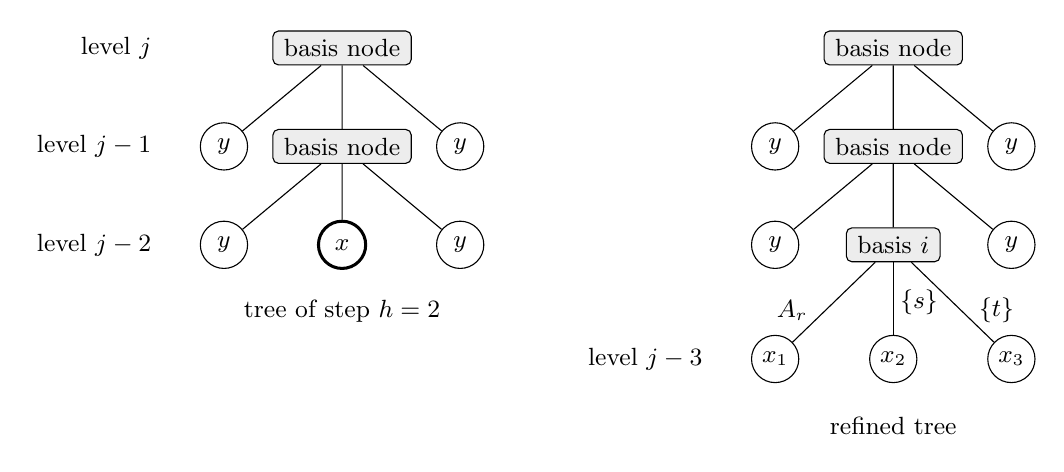
\begin{tikzpicture}[x=1cm,y=1cm,
   inner/.style={draw=black,fill=black!7,rounded corners=2pt,inner xsep=4pt,inner ysep=3pt,font=\small},
   leaf/.style={draw=black,circle,inner sep=1pt,minimum size=6mm,font=\small},
   marked/.style={leaf,line width=1.1pt},
   every node/.style={font=\small}]
\begin{scope}
 \node[inner] (r) at (0,0) {basis node};
 \node[leaf] (r1) at (-1.5,-1.25) {$y$};
 \node[inner] (m) at (0,-1.25) {basis node};
 \node[leaf] (r3) at (1.5,-1.25) {$y$};
 \node[leaf] (m1) at (-1.5,-2.5) {$y$};
 \node[marked] (m2) at (0,-2.5) {$x$};
 \node[leaf] (m3) at (1.5,-2.5) {$y$};
 \draw (r)--(r1) (r)--(m) (r)--(r3) (m)--(m1) (m)--(m2) (m)--(m3);
 \node[anchor=east] at (-2.3,0) {level $j$};
 \node[anchor=east] at (-2.3,-1.25) {level $j-1$};
 \node[anchor=east] at (-2.3,-2.5) {level $j-2$};
 \node at (0,-3.35) {tree of step $h=2$};
\end{scope}
\begin{scope}[xshift=7.0cm]
 \node[inner] (r) at (0,0) {basis node};
 \node[leaf] (r1) at (-1.5,-1.25) {$y$};
 \node[inner] (m) at (0,-1.25) {basis node};
 \node[leaf] (r3) at (1.5,-1.25) {$y$};
 \node[leaf] (m1) at (-1.5,-2.5) {$y$};
 \node[inner] (n) at (0,-2.5) {basis $i$};
 \node[leaf] (m3) at (1.5,-2.5) {$y$};
 \node[leaf] (n1) at (-1.5,-3.95) {$x_1$};
 \node[leaf] (n2) at (0,-3.95) {$x_2$};
 \node[leaf] (n3) at (1.5,-3.95) {$x_3$};
 \draw (r)--(r1) (r)--(m) (r)--(r3) (m)--(m1) (m)--(n) (m)--(m3);
 \draw (n)-- node[left=3pt,pos=.6] {$A_r$} (n1);
 \draw (n)-- node[right=-1pt,pos=.55] {$\{s\}$} (n2);
 \draw (n)-- node[right=3pt,pos=.6] {$\{t\}$} (n3);
 \node[anchor=east] at (-2.3,-3.95) {level $j-3$};
 \node at (0,-4.8) {refined tree};
\end{scope}
\end{tikzpicture}
\caption{The presentation trees in the proof of Theorem~\ref{thm:dimension}, drawn for $h=2$. Left: the tree of step $h$. Its internal nodes are $h$ ternary basis nodes. The marked leaf (bold circle) carries the variable $x$, and the $2h$ side leaves carry the side variable $y$. Right: the refined tree. The marked leaf is replaced by a basis node at a basis $i$, labeled ``basis $i$'', with a ternary template $\{A_r,\{s\},\{t\}\}$; its three children carry independent variables. If the child on $\{s\}$ becomes the marked leaf and the other two children become side leaves, the result is the tree of step $h+1$.}
\label{fig:refinement}
\end{figure}

\begin{proof}[Proof of Theorem~\ref{thm:dimension}]
We construct projections $\Pi_0=I,\Pi_1,\ldots,\Pi_j$ on $\C^d$ such that
\[
 \rank\Pi_{h+1}=\tfrac14\rank\Pi_h\qquad(0\le h\le j-1).
\]
Then $\rank\Pi_j=d/4^j$ is an integer, which proves $4^j\mid d$ for $G_{j,R}$. Each $\Pi_h$ is a coordinate projection~\eqref{eq:coordinate-projection}, and the step from $\Pi_h$ to $\Pi_{h+1}$ recovers the relations of the Mermin--Peres square on the range of $\Pi_h$.

\emph{The tree of step $h$.} All presentation trees in this proof have their root at level $j$, so that they present vertices of $S^j_\lambda(K_3)$. Let $0\le h\le j-1$. The tree of step $h$ has $h$ internal nodes. They are ternary basis nodes at the levels $j,j-1,\ldots,j-h+1$, each a child of the one above it (Figure~\ref{fig:refinement}, left). One leaf, at level $j-h$, is the \emph{marked leaf}; it is a child of the lowest basis node, or the whole tree if $h=0$. The other $2h$ leaves are the \emph{side leaves}. Every leaf is a scalar, padded to the level at which it sits. We assign a variable $x\in\mathbb Z/3$ to the marked leaf and one common variable $y\in\mathbb Z/3$, the \emph{side variable}, to all side leaves. The tree has $h\le2j-1$ internal nodes and no wire node, so it satisfies the bounds of Definition~\ref{def:sparse-graph}. By Fact~1, it defines a graph homomorphism
\[
 F_h:K_3^{\times2}\to G_{j,R},\qquad (y,x)\mapsto F_h(y,x).
\]
The \emph{marked projection} is the coordinate projection of the marked leaf, $\Pi_h=S_{F_h}(\{x\})$. For $h=0$ there are no side leaves, $F_0$ depends only on $x$, and $\Pi_0=I$. The trees of the steps $h\ge1$ are specified at the end of the proof.

\emph{Refining the marked leaf.} Choose a basis $i\in\{1,\ldots,6\}$ and a ternary template $\{A_r,\{s\},\{t\}\}$ at $i$. Replace the marked leaf, which sits at level $j-h\ge1$, by a basis node with this template whose three children are leaves (Figure~\ref{fig:refinement}, right). Assign independent variables $x_1,x_2,x_3\in\mathbb Z/3$ to the children on $A_r$, $\{s\}$ and $\{t\}$, and keep $y$ on the side leaves. The refined tree has $h+1\le j\le2j-1$ internal nodes and no wire node, so by Fact~1 it defines a graph homomorphism $K_3^{\times4}\to G_{j,R}$; for $h=0$ the variable $y$ does not occur. We call the coordinate projections of $x_1,x_2,x_3$ the \emph{child projections} on $A_r$, $\{s\}$ and $\{t\}$. We prove three claims about them and then count ranks.
\begin{list}{}{\setlength{\labelwidth}{3.6em}\setlength{\labelsep}{0.6em}\setlength{\leftmargin}{4.2em}\setlength{\itemsep}{3pt}\setlength{\parsep}{0pt}\setlength{\topsep}{4pt}}
\item[\textup{Claim 1.}] For every basis $i$ and every ternary template at $i$, the three child projections are pairwise orthogonal and sum to $\Pi_h$.
\item[\textup{Claim 2.}] Fix a basis $i$. For $s\in\{1,2,3\}$, the child projection on the singleton $\{s\}$ is the same for the two ternary templates at $i$ that contain $\{s\}$; we denote it by $T^i_s$. With $T^i_0=\Pi_h-T^i_1-T^i_2-T^i_3$, the operators $T^i_0,T^i_1,T^i_2,T^i_3$ are pairwise orthogonal projections with sum $\Pi_h$, and the child projection on $A_r$ is $D^i_r=T^i_0+T^i_r$ for $r=1,2,3$.
\item[\textup{Claim 3.}] Let $e=ik$ be an edge of $K_{3,3}$ with $A_{i,e}=A_r$. If $e\ne36$ and $A_{k,e}=A_{r'}$, then $D^i_r=D^k_{r'}$. For the complemented edge, $D^3_3=\Pi_h-D^6_3$.
\end{list}

\emph{Proof of Claim~1.} The three child projections are pairwise orthogonal by Fact~3. For the sum, set $x_1=x_2=x_3=x$. The refined tree then presents a vertex $F^i_h(y,x)$, in which the marked leaf is replaced by the constant word on $x$ in basis $i$. By Fact~5, the three child projections sum to the coordinate projection of $x$ for the homomorphism $F^i_h$. It therefore suffices to show that
\[
 P_{F^i_h(y,x),a}=P_{F_h(y,x),a}\qquad\text{for all }y,x,a\in\mathbb Z/3\text{ and every basis }i.
\]
For $i=6$ this holds because the constant word on $x$ in basis $6$ is the padding of the scalar $x$, so that $F^6_h=F_h$. Now let $e=ik$ be an edge of $K_{3,3}$. For each layer $\ell\in\{0,\ldots,\lambda+1\}$, replace the marked leaf by a wire node on $e$ at layer $\ell$ whose two children are both the scalar leaf $x$. This tree has $h+1\le2j-1$ internal nodes, one of them a wire node with a scalar background, so it satisfies Definition~\ref{def:sparse-graph}. At the layers $0$ and $\lambda+1$ it presents $F^i_h(y,x)$ and $F^k_h(y,x)$. By Fact~2, the homomorphisms of two consecutive layers satisfy the cross-edge condition, so by Fact~7 they carry the same measurements. Hence so do $F^i_h$ and $F^k_h$. Since $K_{3,3}$ is connected, the measurements of every $F^i_h$ agree with those of $F^6_h=F_h$.

\emph{Proof of Claim~2.} Let $s\in\{1,2,3\}$, and consider one of the two ternary templates at $i$ that contain $\{s\}$. Set the variable of the child on $\{s\}$ equal to $x$ and the variables of the other two children equal to $y$. By Fact~5, this identification leaves the child projection on $\{s\}$ unchanged: it becomes the coordinate projection of $x$ for the resulting homomorphism $K_3^{\times2}\to G_{j,R}$. The vertex that this homomorphism presents has, in place of the marked leaf, the word of basis $i$ with $x$ at position $s$ and $y$ at the other three positions. This word is the same for both templates, so the child projection on $\{s\}$ does not depend on the template. Two distinct positions $s,t\in\{1,2,3\}$ are singleton parts of one template $\{A_r,\{s\},\{t\}\}$. By Claim~1, the projections $T^i_s$ and $T^i_t$ are therefore orthogonal, and both lie below $\Pi_h$. Hence $T^i_0$ is a projection, and $T^i_0,T^i_1,T^i_2,T^i_3$ are pairwise orthogonal with sum $\Pi_h$. Finally, by Claim~1 the child projection on $A_r$ equals $\Pi_h-T^i_s-T^i_t=T^i_0+T^i_r$.

\emph{Proof of Claim~3.} Let $e=ik$ be an edge of $K_{3,3}$ with $i\le3<k$. For each layer $\ell\in\{0,\ldots,\lambda+1\}$, replace the marked leaf by a wire node on $e$ at layer $\ell$ whose first child is a leaf with the variable $x$ and whose background is a leaf with the side variable $y$. As in the proof of Claim~1, these trees satisfy Definition~\ref{def:sparse-graph}. By Facts~2 and~7, the measurements are the same at all layers, and so is the coordinate projection of $x$. At layer $0$ the tree presents the word of basis $i$ with $x$ on $A_{i,e}=A_r$ and $y$ on the complement. As in the proof of Claim~2, the coordinate projection of $x$ is then the child projection on $A_r$ at basis $i$, which is $D^i_r$. At layer $\lambda+1$ the tree presents the word of basis $k$ with $x$ on $A_{k,e}$ and $y$ on the complement. If $e\ne36$ and $A_{k,e}=A_{r'}$, the coordinate projection of $x$ is $D^k_{r'}$ for the same reason. If $e=36$, then $x$ occupies $A_{6,36}=A_3^c=\{1,2\}$ and $y$ occupies $A_3$. For the template $\{A_3,\{1\},\{2\}\}$ this is the word whose two singleton children both carry $x$, so the coordinate projection of $x$ is $T^6_1+T^6_2=\Pi_h-D^6_3$.

\emph{The relations of the square.} By Claim~2, the operators
\[
 L^i_r=2D^i_r-\Pi_h\qquad(r=1,2,3)
\]
are self-adjoint involutions on the range of $\Pi_h$. They commute pairwise and satisfy $L^i_1L^i_2L^i_3=\Pi_h$: on the range of $T^i_0$ all three equal $+1$, and on the range of $T^i_s$ with $s\ge1$ the involution $L^i_r$ equals $+1$ for $r=s$ and $-1$ for $r\ne s$. In particular, the ranges of $T^i_0,T^i_1,T^i_2,T^i_3$ are the four joint eigenspaces of any two of $L^i_1,L^i_2,L^i_3$. By Claim~3, an edge $e=ik$ with $A_{i,e}=A_r$ and $A_{k,e}=A_{r'}$ gives $L^i_r=L^k_{r'}$ if $e\ne36$, and the complemented edge gives $L^3_3=-L^6_3$.

Arrange the nine involutions of the row bases in a $3\times3$ array: for an edge $e=ik$ with $A_{i,e}=A_r$, put $L^i_r$ in row $i\in\{1,2,3\}$ and column $k\in\{4,5,6\}$. Row $i$ consists of $L^i_1,L^i_2,L^i_3$, because the three edges at basis $i$ use $A_1,A_2,A_3$ once each (Table~\ref{tab:edges}). Its entries commute, and their product is $+\Pi_h$. By the relations just stated, column $k\in\{4,5\}$ consists of $L^k_1,L^k_2,L^k_3$, and column $6$ consists of $L^6_1$, $L^6_2$ and $-L^6_3$. Hence the entries of every column commute, columns $4$ and $5$ have product $+\Pi_h$, and column $6$ has product $-\Pi_h$. These are the relations of the array~\eqref{eq:pauli-square}. Negating the two entries of row $1$ in columns $4$ and $5$ leaves all row products equal to $+\Pi_h$ and makes all three column products equal to $-\Pi_h$. Call the resulting array $U$.

\emph{Counting ranks.} Lemma~\ref{lem:square-rank}, applied on the range of $\Pi_h$, shows that the four joint eigenspaces of any two distinct entries in a row or in a column of $U$ have equal dimension. Two entries of row $i$ are $\pm L^i_r$ and $\pm L^i_{r'}$ with $r\ne r'$, and two entries of column $k$ are $\pm L^k_r$ and $\pm L^k_{r'}$ with $r\ne r'$. In both cases the four joint eigenspaces are the ranges of $T^b_0,T^b_1,T^b_2,T^b_3$ for the basis $b$ in question. Therefore, for every basis $i\in\{1,\ldots,6\}$,
\begin{equation}\label{eq:quarter-rank}
 \rank T^i_s=\tfrac14\rank\Pi_h\qquad (0\le s\le3).
\end{equation}

\emph{The next step.} Choose a basis $i$ and a ternary template $\{A_r,\{s\},\{t\}\}$ at $i$, and refine the marked leaf accordingly. In the refined tree, let the child on $\{s\}$ be the new marked leaf, with the variable $x$, and let the children on $A_r$ and $\{t\}$ be side leaves, with the variable $y$. As in the proof of Claim~2, the marked projection of this tree is $T^i_s$. We put $\Pi_{h+1}=T^i_s$, so that $\rank\Pi_{h+1}=\frac14\rank\Pi_h$ by~\eqref{eq:quarter-rank}. If $h+1\le j-1$, this tree is the tree of step $h+1$, and the construction continues. Starting from $\Pi_0=I$, we obtain $\rank\Pi_j=d/4^j$ after $j$ steps, which proves $4^j\mid d$ for $G_{j,R}$.

Because every quantum $3$-coloring of $S^j_\lambda(K_3)$ restricts to the induced subgraph $G_{j,R}$, $4^j\mid d$ also holds for $S^j_\lambda(K_3)$. Conversely, Theorems~\ref{thm:gap} and~\ref{thm:sparse} supply an $R$-compatible quantum $3$-coloring of both graphs in local dimension $4^j$, and taking direct sums produces $R$-compatible quantum $3$-colorings in every positive multiple of $4^j$.
\end{proof}

The magic square game is known to self-test two EPR pairs because its perfect strategies are rigid up to local isometries~\cite{WBMS,CS}. Theorem~\ref{thm:dimension} establishes an analogous rigidity statement for the graph coloring game at the level of local dimension: every quantum $3$-coloring of $G_{j,R}$ or $S^j_\lambda(K_3)$ must embed the algebraic relations of the Mermin--Peres square $j$ times in succession, regardless of compatibility.

\subsection{Exact compatibility radius and proof of the main theorem}\label{sec:largest-radius}

The involutions recovered at step $h=0$, where $\Pi_0=I$, also show that no quantum $3$-coloring of $G_{j,R}$ or $S^j_\lambda(K_3)$ can commute beyond distance $\max\{R,2\}$.

\begin{proposition}\label{prop:largest-compatible-radius}
For all $j,R\ge1$, the largest integer $k$ for which $G_{j,R}$ admits a $k$-compatible quantum $3$-coloring is $\lambda+2=\max\{R,2\}$, where $\lambda=\max\{R-2,0\}$. The same holds for the full iterate $S^j_\lambda(K_3)$.
\end{proposition}
\begin{proof}
By Theorems~\ref{thm:gap} and~\ref{thm:sparse}, the displayed coloring is $(\lambda+2)$-compatible on both $S^j_\lambda(K_3)$ and $G_{j,R}$.

For the upper bound, let $(P_{v,a})$ be an arbitrary finite-dimensional quantum $3$-coloring of $G_{j,R}$ on $\C^d$. Consider step $h=0$ of the proof of Theorem~\ref{thm:dimension}, where $\Pi_0=I$, and its two involutions
\[
 L^1_2=2D^1_2-I,\qquad L^4_1=2D^4_1-I.
\]
By Table~\ref{tab:edges}, $L^1_2$ belongs to the edge $15$ and stands in row $1$ and column $5$ of the array of involutions. By Claim~3 of that proof, $L^4_1=L^2_2$, which belongs to the edge $24$ and stands in row $2$ and column $4$. Up to sign, these are two entries of the array $U$ in distinct rows and distinct columns. Such entries anticommute by Lemma~\ref{lem:square-rank}, and a change of sign does not affect this. Hence $L^1_2L^4_1=-L^4_1L^1_2$.

We recover $D^1_2$ and $D^4_1$ from four concrete vertices of $G_{j,R}$. Write each entry below for a scalar padded to level $j-1$ in basis $6$:
\[
\begin{array}{c|cc}
 &\text{constant word}&\text{two-label word}\\ \hline
 \text{basis }1&r_0=(1,1,1,1)&r_1=(1,0,1,0)\\
 \text{basis }4&c_0=(2,2,2,2)&c_1=(2,2,1,1).
\end{array}
\]
The vertices $r_0,r_1$ belong to the ternary template with doubleton $A_2=\{0,2\}$ in basis $1$, and $c_0,c_1$ belong to the ternary template with doubleton $A_1=\{0,1\}$ in basis $4$. By Fact~4, a coordinate projection may be evaluated using any two distinct color labels (here $1$ and $0$ for $D^1_2$, and $2$ and $1$ for $D^4_1$), yielding
\[
 D^1_2=\sum_{a\in\mathbb Z/3} P_{r_0,a}P_{r_1,a},\qquad
 D^4_1=\sum_{a\in\mathbb Z/3} P_{c_0,a}P_{c_1,a}.
\]

We now bound $\dist_{G_{j,R}}(r_i,c_{i'})$ for all $i,i'\in\{0,1\}$. In basis $1$, both $r_0$ and $r_1$ avoid color $2$ in all four positions, so both are adjacent to the constant word $u_1=(2,2,2,2)$ in basis $1$. Similarly, in basis $4$, both $c_0$ and $c_1$ avoid color $0$ in all four positions, so both are adjacent to the constant word $u_4=(0,0,0,0)$ in basis $4$. Along wire $14$, we join $u_1$ (layer $0$) to $u_4$ (layer $\lambda+1$) by a path of $\lambda+1$ edges. To this end, take any walk $a_0,a_1,\ldots,a_{\lambda+1}$ in $K_3$ of length $\lambda+1$ with $a_0=2$ and $a_{\lambda+1}=0$, and place the equal pair $(a_\ell,a_\ell)$, padded to level $j-1$, at layer $\ell$. Such a walk exists for every $\lambda+1\ge1$: lengths $1$ and $2$ use $2,0$ and $2,1,0$, and any walk extends by two steps via a single backtrack. Every basis word and wire vertex along this path admits a presentation with $1$ internal node and at most $1$ wire node, hence lies in $G_{j,R}$ for every $j\ge1$. Therefore
\[
 \dist_{G_{j,R}}(r_i,c_{i'})\le 1+(\lambda+1)+1=\lambda+3\qquad (i,i'\in\{0,1\}).
\]

If $(P_{v,a})$ were $(\lambda+3)$-compatible, every projector at $r_0$ or $r_1$ would commute with every projector at $c_0$ or $c_1$. Then $D^1_2$ and $D^4_1$, and hence $L^1_2$ and $L^4_1$, would commute. Because $L^1_2$ and $L^4_1$ are involutions on the nonzero space $\C^d$, their product is invertible, which contradicts $L^1_2L^4_1=-L^4_1L^1_2$. Thus no quantum $3$-coloring of $G_{j,R}$ is $(\lambda+3)$-compatible. Finally, because distances in the induced subgraph $G_{j,R}$ are at least distances in the full iterate $S^j_\lambda(K_3)$, any $k$-compatible coloring of $S^j_\lambda(K_3)$ restricts to a $k$-compatible coloring of $G_{j,R}$, proving the same upper bound $\lambda+2$ for $S^j_\lambda(K_3)$.
\end{proof}

For $R\ge2$, Proposition~\ref{prop:largest-compatible-radius} states that the compatibility radius of $G_{j,R}$ and $S^j_\lambda(K_3)$ is exactly $R$: no choice of quantum strategy on these graphs can commute further. When $R\in\{1,2\}$, we have $\lambda=0$, so $G_{j,1}=G_{j,2}$ and their compatibility radius is exactly $2$.

Every ingredient of Theorem~\ref{thm:main} is now established, and we assemble its proof.

\begin{proof}[Proof of Theorem~\ref{thm:main}]
Let $j,R\ge1$, $\lambda=\max\{R-2,0\}$, and $G=S^j_\lambda(K_3)$. Theorem~\ref{thm:gap} establishes $\cq(G)=3$, $\chi(G)\ge2j+3$, and a $(\lambda+2)$-compatible, hence $R$-compatible, quantum $3$-coloring in local dimension $4^j$. As explained in Section~\ref{sec:sparse} using~\eqref{eq:pauli-square}, this strategy consists of adaptive two-qubit Pauli measurements on $2j$ EPR pairs, proving~(i). Theorem~\ref{thm:dimension} proves~(ii), that every finite-dimensional quantum $3$-coloring of $G$ has local dimension divisible by $4^j$, assuming only the edge rule. Proposition~\ref{prop:largest-compatible-radius} proves~(iii), that no quantum $3$-coloring of $G$ is $k$-compatible for any $k>\max\{R,2\}$. Finally, Theorem~\ref{thm:sparse} provides the explicit induced subgraph $G_{j,R}$ of $G$. It satisfies $\cq(G_{j,R})=3$, $\chi(G_{j,R})\ge2j+3$ and $|V(G_{j,R})|+|E(G_{j,R})|\le[C(1+R)]^j$ for an absolute constant $C$, and the adaptive Pauli coloring restricts to an $R$-compatible quantum $3$-coloring of $G_{j,R}$ in local dimension $4^j$. Theorem~\ref{thm:dimension} and Proposition~\ref{prop:largest-compatible-radius} establish~(ii) and~(iii) directly for $G_{j,R}$ as well, which proves~(iv).
\end{proof}
